\section{Results}

\begin{table*}[t]
\centering
\small
\begin{minipage}{0.48\textwidth}
\centering
\textbf{Training tasks}\\[2pt]
\begin{tabular}{lrrr}
\toprule
Website & No rules & \expel{}-style & Reflection \\
\midrule
V1.45.0 & 9/68 & 56/68 & -- \\
V2 & -- & 60/68 & 67/68 \\
V3 & -- & 8/68 & 65/68 \\
\bottomrule
\end{tabular}
\end{minipage}
\hfill
\begin{minipage}{0.48\textwidth}
\centering
\textbf{Held-out validation tasks}\\[2pt]
\begin{tabular}{lrrr}
\toprule
Website & No rules & \expel{}-style & Reflection \\
\midrule
V1.45.0 & 133/167 & 124/167 & -- \\
V2 & -- & 114/167 & 143/167 \\
V3 & -- & 66/167 & 97/167 \\
\bottomrule
\end{tabular}
\end{minipage}
\caption{Overall success counts across website versions. \expel{}-style rules help on \linkding{} V1.45.0 but degrade under harder website drift. Reflection rules remain stronger on the generated website suites. Detailed per-drift results for R1--R4 on website V3 are reported in Appendix Tables~\ref{tab:training_v3_appendix} and~\ref{tab:heldout_v3_appendix}.}
\label{tab:website_version_summary}
\end{table*}

\begin{figure*}[t]
\centering
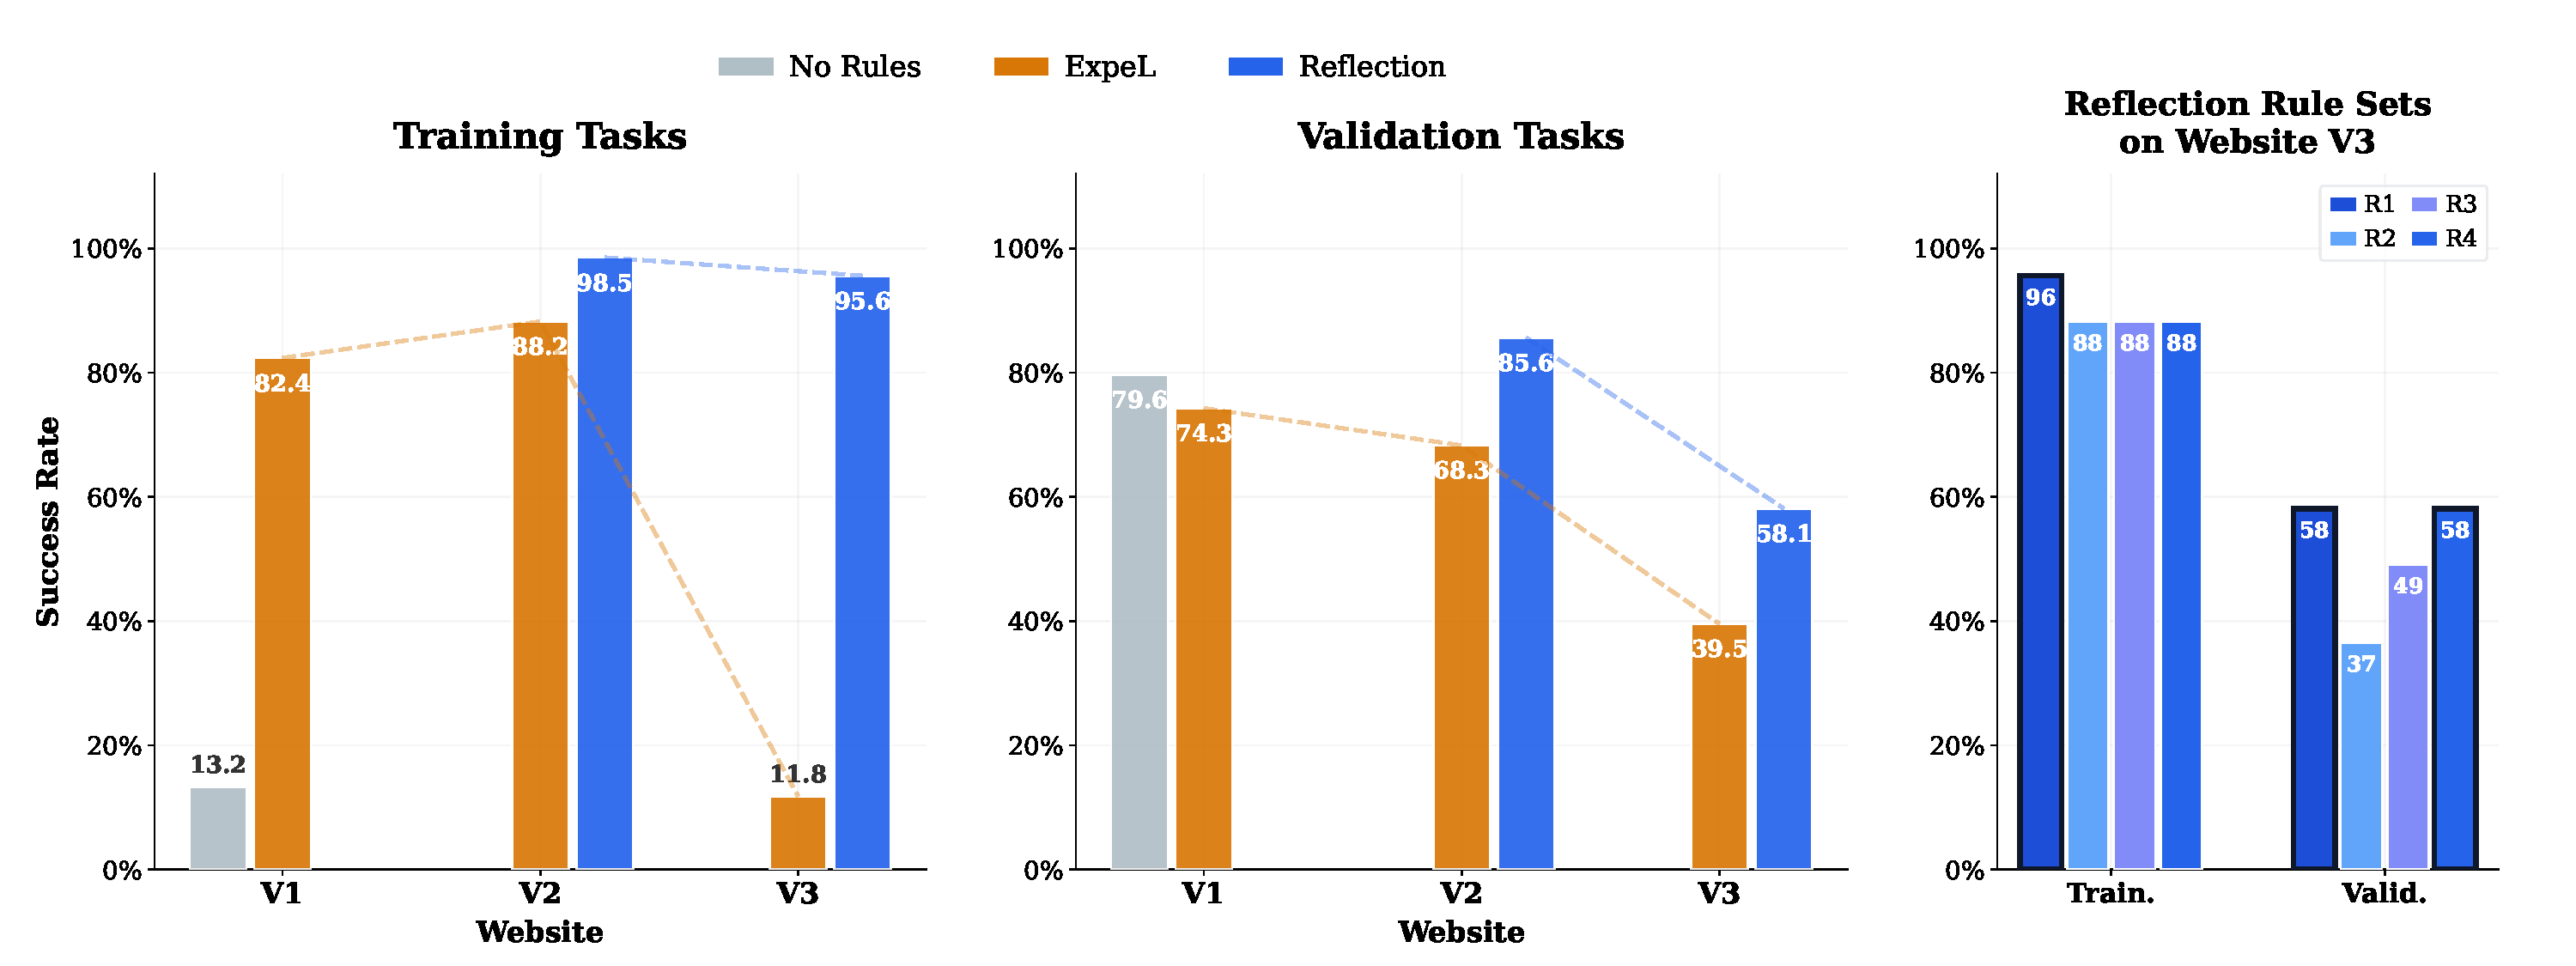
\includegraphics[width=\textwidth]{output/poster_fig_a_hero.pdf}
\caption{Headline robustness results across website versions. The left and middle panels compare no rules, \expel{}-style rules, and the strongest available reflection-rule condition on the training and held-out validation tasks. The right panel isolates the website V3 reflection-rule sets R1--R4, showing that later rule revisions are not monotonically better.}
\label{fig:website_version_overview}
\end{figure*}

\begin{table}[t]
\centering
\small
\begin{tabular}{lcc}
\toprule
Rules & Training & Held-out \\
\midrule
R1 & 65/68 (95.6\%) & 97/167 (58.1\%) \\
R2 & 60/68 (88.2\%) & 97/167 (58.1\%) \\
R3 & 60/68 (88.2\%) & 61/167 (36.5\%) \\
R4 & 60/68 (88.2\%) & 82/167 (49.1\%) \\
\bottomrule
\end{tabular}
\caption{Overall website V3 success for successive reflection-rule sets. R1--R4 are obtained through iterative reflection on observed failures and rule revision; detailed per-drift counts are deferred to Appendix Tables~\ref{tab:training_v3_appendix} and~\ref{tab:heldout_v3_appendix}.}
\label{tab:v3_reflection_overall}
\end{table}


\paragraph{Experimental setting.}
We evaluate a fixed multimodal web agent on a self-hosted bookmark-management website under three conditions: no retrieved rules, \expel{}-style rules~\citep{zhao2023expel}, and \expel{}-style rules augmented with reflection rules. The evaluation uses 68 training tasks for diagnosing rule behavior and 167 held-out validation tasks for testing transfer to unseen task families. We report task success rate on \linkding{} V1.45.0, on a moderately modified website V2, and on a harder generated website suite V3 that changes access, visual presentation, content, timing, workflow, navigation structure, and feature affordances while preserving the user goal. For website V3, R1--R4 denote successive reflection-rule sets obtained through iterative reflection on observed failures and rule revision.

\subsection{\expel{}-Style Rules Help, but Do Not Fully Transfer}

On \linkding{} V1.45.0, \expel{}-style rules provide a strong training-task gain: success increases from \(13.2\%\) without rules to \(82.4\%\) with retrieved \expel{}-style rules. This confirms that reusable experience is a meaningful starting point rather than a weak baseline. The same rules, however, do not uniformly improve held-out behavior. On held-out validation tasks from \linkding{} V1.45.0, success changes from \(79.6\%\) without rules to \(74.3\%\) with \expel{}-style rules. This motivates separating training tasks from held-out validation tasks instead of reporting a single averaged score.

\subsection{Reflection Rules Help Under Moderate Website Drift}

We next test whether reflection rules add value when the website changes but the task goals remain the same. On website V2, adding reflection rules improves the training tasks from \(88.2\%\) to \(98.5\%\), and improves the held-out validation tasks from \(68.3\%\) to \(85.6\%\) (Table~\ref{tab:website_version_summary} and Figure~\ref{fig:website_version_overview}). Since the model, tasks, website version, and \expel{}-style rules are held fixed, these gains isolate the benefit of rules that describe how to preserve intent across interface changes.

\subsection{Website V3 Exposes the Robustness Gap}

The harder generated website suite V3 creates the main robustness stress test. With \expel{}-style rules alone, success drops to \(11.8\%\) on the training tasks. The strongest reflection-rule set recovers performance to \(95.6\%\), while three alternative rule sets reach \(88.2\%\) (Table~\ref{tab:v3_reflection_overall}). Figure~\ref{fig:v3_drift_rule_profile} shows that the recovery is broad across drift families rather than coming from a single easy bucket. This large gap shows that robustness under website drift is not obtained simply by adding more task-level guidance; the useful rules are those that explicitly describe how to recover from changed navigation paths, delayed readiness, changed labels, and shifted workflow cues.

The held-out validation tasks remain substantially harder. \expel{}-style rules alone reach \(39.5\%\). The two strongest reflection-rule sets, R1 and R4, reach \(58.1\%\), while weaker variants R3 and R2 reach \(49.1\%\) and \(36.5\%\). Thus, reflection rules improve transfer under harder drift, but the gains are uneven: a plausible rule update can improve one family of failures while regressing another.

\subsection{Rule Updates Are Useful but Non-Monotonic}

The detailed website V3 matrices in Appendix Tables~\ref{tab:training_v3_appendix} and~\ref{tab:heldout_v3_appendix}, summarized visually in Figure~\ref{fig:v3_reflection_iteration} and Figure~\ref{fig:v3_drift_rule_profile}, show that the best aggregate reflection-rule set is not simply the most recent edit. One evidence-based update improves several held-out drift categories, including authentication-related, visual, content, and timing changes, but loses ground on workflow and feature-affordance changes. The aggregate tie on the held-out validation tasks therefore hides a real tradeoff between different recovery behaviors.

This pattern supports the main design choice in \webcoevo{}: rule generation, verification, and promotion should be separate stages. Matched trajectories can suggest useful edits, but an edit should not be promoted only because it is plausible or locally evidence-grounded. It must also preserve previously successful behaviors under the same website-drift distribution.

\subsection{Failure Analysis: Why Iterative Reflection Degrades Held-Out Generalization}
\label{sec:failure_analysis}

The per-drift breakdown in Appendix Tables~\ref{tab:training_v3_appendix} and~\ref{tab:heldout_v3_appendix} exposes a sharp asymmetry between training and held-out behavior. On the 68 training tasks, successive rule sets differ modestly: R1 reaches \(65/68\) and R2--R4 each reach \(60/68\). On the 167 held-out tasks, the same transition produces a collapse: R1 achieves \(97/167=58.1\%\), R2 falls to \(61/167=36.5\%\)---\emph{below} the \expel{}-only baseline of \(66/167=39.5\%\)---and R3 and R4 partially recover to \(82/167=49.1\%\) and \(97/167=58.1\%\). The training-to-held-out loss ratio from R1 to R2 is approximately \(7{\times}\): five tasks lost on training compared with thirty-six on held-out. This ratio is not consistent with stochastic noise; it reflects a structural difference in how the reflection loop interacts with its evidence source.

\paragraph{The general finalization rule: presence, removal, and restoration.}
Inspection of the rulebook diffs pinpoints the dominant mechanism. R1 includes a broadly scoped rule covering seven drift types, including \texttt{process}, \texttt{functional}, and \texttt{access}: \emph{``Finalize instead of noop when URL, query, or heading already proves the target state.''}
During the R1$\to$R2 iteration, the reflection generator encountered evidence of agents over-committing to staged review checkpoints and produced a replacement rule scoped identically across the same seven drift types: \emph{``Treat staged review or apply pages as one-click checkpoints, not as noop states.''}
This substitution is locally coherent---the new rule addresses a real failure mode observed in training traces---but it silently removes the general finalization signal. For the fourteen process task instances in the held-out set, the agent now receives three rules, none of which advises it when multi-step evidence in the URL or heading is sufficient to stop. The result is that all fourteen process tasks that R1 handled correctly exhaust the maximum step budget (\texttt{max\_steps\_no\_success}), dropping held-out process success from \(13/19=68.4\%\) to \(5/19=26.3\%\). The same removal affects held-out \texttt{functional} tasks, which fall from \(7/13=53.8\%\) to \(3/13=23.1\%\). R4 explicitly restores the finalization principle in a slightly generalized form---\emph{``Finalize instead of acting when URL, query, heading, or redirected destination already proves completion''}---explaining why R4 recovers the aggregate held-out score to R1's level.

\paragraph{Completion-signal tightening in filtered bookmark tasks.}
A related substitution compounds the functional degradation. R1 instructs the agent to \emph{``treat query-state arrival as completion evidence''} for filtered bookmark tasks. The R2 iteration, having observed cases where agents prematurely finalized on pre-filter states, tightens this to \emph{``distinguish prepared lookup states from committed filter results.''} For the training tasks, this distinction is well-grounded: the agent was genuinely confusing two observable states. For unseen held-out task variants that do not share the same two-state structure, the tightened rule introduces hesitation at moments when the R1 rule would have accepted completion. This contributes to the functional regression and persists through R3, which applies a similarly conservative phrasing (\emph{``finalize exact query evidence before apply or commit recovery''}), before R4 explicitly restores the original completion-signal wording.

\paragraph{Content drift: where ExpeL experience dominates.}
A structurally different failure appears in the \texttt{content} bucket, where \expel{}-style rules achieve \(11/14=78.6\%\) on held-out tasks but every reflection-augmented version underperforms: R1 drops to \(7/14=50.0\%\), and even R4 recovers only to \(10/14=71.4\%\), still below the \expel{} baseline. \texttt{Content} drift re-labels interface elements while preserving the underlying data model and task logic, so success requires generalizing over surface-token variation without task-specific anchors. \expel{}-style rules, derived from cross-task trajectory experience accumulated over many task families, encode this tolerance implicitly. Reflection rules, constructed from failure traces on specific training-content variants, encode expectations about particular form labels or placeholder wording; this specificity transfers poorly to held-out content variants that use different surface tokens but identical task structure.

\paragraph{Asymmetric recovery and the cost of semantic abstraction.}
R3 and R4 recover the categories with observable, page-level failure signals---\texttt{access} rises from \(3/36=8.3\%\) under R2 to \(12/36=33.3\%\) under R3, and \texttt{surface} rises from \(19/36=52.8\%\) to \(30/36=83.3\%\) under R4---because URL mismatch and missing entry-point evidence are straightforward to diagnose from trajectory data. The categories that require semantic reasoning (\texttt{process}, \texttt{functional}, \texttt{structural}) plateau across R3 and R4 at levels persistently below R1, confirming that the reflection loop's evidence-grounded repair process is well-suited to correcting observable navigation failures but systematically ill-suited to restoring abstract behavioral principles once they have been displaced by iteration-specific patches.

\paragraph{Root cause: locally grounded reflection without generalization constraints.}
The trace-level evidence across R1--R4 points to a single structural limitation. Each reflection iteration receives failure evidence drawn exclusively from training tasks and proposes rule edits that are locally consistent with that evidence. The resulting rulebook can pass training-distribution checks while silently degrading the abstract, broadly scoped rules that govern held-out transfer. No component of the current reflection loop's prompt---not the failure-case selector, the rule editor, nor the verification stage---explicitly evaluates whether a proposed substitution narrows a general behavioral principle into a training-specific patch. The \(7{\times}\) training-to-held-out loss ratio at the R1$\to$R2 transition, and the need for R4 to manually restore rules that R1 had already learned, both indicate that promoting a rule because it is locally plausible is insufficient; a sound reflection loop must additionally verify that the promotion does not remove coverage for held-out conditions the training distribution does not expose. Appendix~\ref{sec:case_studies} presents three trace-level case studies that instantiate each failure mode with concrete step sequences and rule diffs.
